
\section*{Schaalafhankelijke æther dichtheid in het Vortex Æther Model (VAM)}


VAM gebruikt een schaalafhankelijke ætherdichtheid: lokaal zeer hoog ($\sim10^{18}$ kg/m³) voor kernstabiliteit en macroscopisch laag ($\sim10^{-7}$ kg/m³) om inertievrije propagatie van interacties mogelijk te maken. De hoge dichtheid in wervelkernen versterkt lokaal de wervelsnelheid en daarmee de tijddilatatie significant, terwijl macroscopisch juist minimale weerstand voor propagatie van effecten geboden wordt.


In het Vortex Æther Model (VAM) wordt de ætheropgevat als een superfluide, onviskeuze continu"um met constante dichtheid binnen macroscopische gebieden, maar met een \emph{schaalafhankelijke structuur} rondom vortexknopen. Deze structuur vereist een hoge lokale dichtheid nabij de kern voor stabiliteit, en een ijle ætherop grote schaal om vrije propagatie van signalen (zoals licht) mogelijk te maken.

\subsection*{1. Kernregime}

De dichtheid in de kern benadert:
\begin{equation}
    \rho_\text{\ae}(r \to 0) \sim \SI{3.89e18}{kg/m^3},
\end{equation}
vereist om topologische stabiliteit van de vortexkern te garanderen. Deze waarde volgt uit energetische argumenten:
\begin{equation}
    E_{\text{vortex}} = \frac{1}{2} \rho_\text{\ae} \Omega^2 r_c^5 \quad\Rightarrow\quad \rho_\text{\ae} \sim \frac{2 E}{\Omega^2 r_c^5},
\end{equation}
waarbij \( \Omega = \frac{C_e}{r_c} \) de kernrotatie is, met \( C_e \approx \SI{1.094e6}{m/s} \) en \( r_c \approx \SI{1.409e-15}{m} \).

\subsection*{2. Overgangsregime}

Voor afstanden groter dan de kern, maar kleiner dan macroschaal, geldt een exponenti"ele afname:
\begin{equation}
    \rho_\text{\ae}(r) = \rho_\text{far} + (\rho_\text{core} - \rho_\text{far}) e^{-r/r_*},
\end{equation}
met \( r_* \sim \SI{1e-12}{m} \) de karakteristieke overgangsschaal. Deze waarde wordt gemotiveerd door het bereik van vortexinvloeden (zoals in EM-interacties).

\subsection*{3. Macroscopisch Regime}

Voor \( r \gg r_* \) bereikt \( \rho_\text{\ae} \) asymptotisch een constante waarde:
\begin{equation}
    \rho_\text{far} \sim \SI{1e-7}{kg/m^3},
\end{equation}
waardoor vrije voortplanting van signalen zonder merkbare inertie optreedt. Dit simuleert een vacu"umachtig gedrag.


\begin{figure}[htbp]
    \centering
    \includegraphics[width=0.85\textwidth]{images/00_scaleDependentÆtherDensity_nl}
    \caption{De ætherdichtheid neemt exponentieel af vanaf de vortexkern en benadert asymptotisch een constante waarde op macroschaal.}
    \label{fig:vortexfields2}
\end{figure}

\begin{table}[h!]
    \centering
    \begin{tabular}{|c|c|c|l|}
        \hline
        Regime & Afstand $r$ & $\rho_\text{\ae}(r)$ & Fysische interpretatie \\
        \hline
        Kern & $r < 10^{-14}$ m & $\sim 10^{18}$ kg/m$^3$ & Vortexstabiliteit \& inertie \\
        Overgang & $10^{-14} - 10^{-11}$ m & Exponentieel dalend & Swirl-uitdoving \& massa-interactie \\
        Macroscopisch & $r > 10^{-11}$ m & $\sim 10^{-7}$ kg/m$^3$ & Vrije ætherzonder massaweerstand \\
        \hline
    \end{tabular}
    \caption{Gedrag van de ætherdichtheid op verschillende schalen.}
\end{table}


\section{Tijddilatatie vanuit wervel dynamiek}

We beschouwen een onzichtbare, rotatievrije superfluïde æther met stabiele topologische wervelknopen. Absolute tijd $t_\text{abs}$ stroomt met een constante snelheid, terwijl lokale klokken mogelijk een lagere snelheid ervaren als gevolg van drukgradiënten en knoopenergetica. Het Vortex Æther Model veronderstelt dat de snelheid waarmee tijd in het lokale frame (dichtbij de knoop) stroomt, afhangt van de interne hoekfrequentie $\Omega_k$. In deze sectie leiden we tijddilatatie-analogen af, geïnspireerd door de voorspellingen van de algemene relativiteitstheorie (GR), uitsluitend gebaseerd op druk- en vorticiteitsgradiënten in de vloeistof.

\begin{figure}[htbp]
\centering
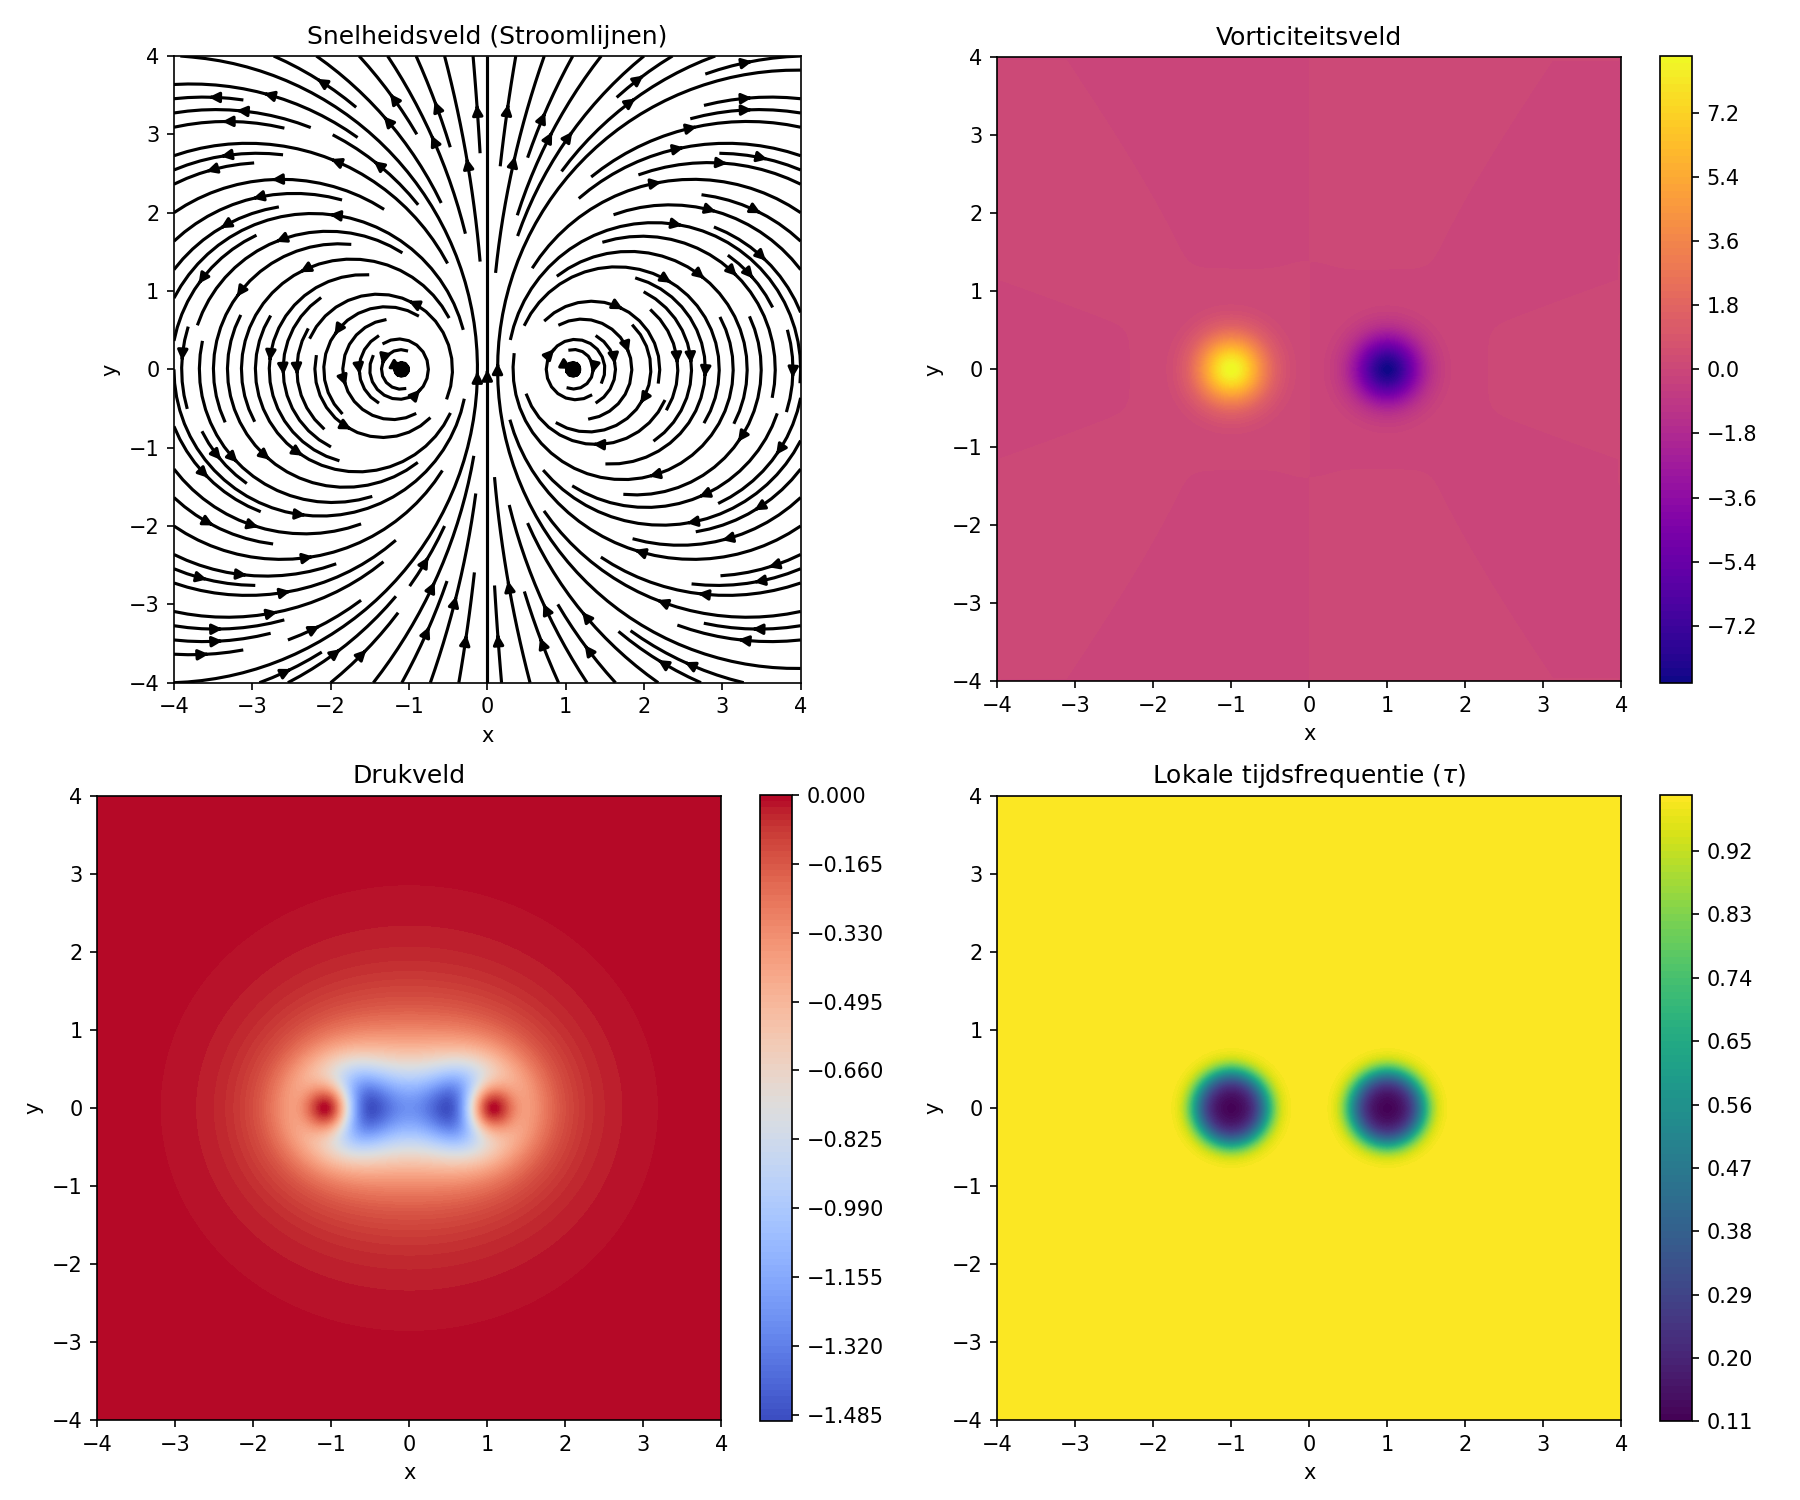
\includegraphics[width=0.85\textwidth]{images/01-streamlinesDiPole_nl}
\caption{Snelheid stroomlijnt, vorticiteit, druk en lokale tijdsnelheid $\tau$ voor een gesimuleerd wervelpaar. Het drukminimum en de tijdvertraging komen duidelijk overeen met de gebieden met hoge vorticiteit. Dit illustreert direct de centrale bewering van het æther model: tijddilatatie volgt uit wervelenergetica en drukvermindering.}
\label{fig:vortexfields}
\end{figure}

In het Vortex Æther Model (VAM) ontstaat tijddilatatie niet vanuit de kromming van ruimtetijd, maar vanuit lokale wervel dynamica. Elk materiedeeltje is in VAM een wervel-knoopstructuur waarvan de interne rotatie (\textit{swirl}) de lokale klokfrequentie beïnvloedt.

De fundamentele koppeling tussen lokale wervel-snelheid en de lokale tijdsmeting volgt uit de Bernoulli-achtige relatie voor drukverlaging in stromingsvelden. De lokale klokfrequentie is gerelateerd aan de wervel-tangentiële snelheid $v_{\phi}(r)$ via de formule:
\begin{equation}\label{eq:vortex_tijddilatatie}
    \frac{d\tau}{dt} = \sqrt{1 - \frac{v_{\phi}^2(r)}{c^2}}
\end{equation}

Hierbij is $v_{\phi}(r)$ de tangentiële snelheid van het æther medium op afstand $r$ tot het centrum van de wervel, en $c$ de lichtsnelheid. Dit is een directe analogie met de speciale relativistische snelheidsafhankelijke tijddilatatie, echter zonder ruimtetijdkromming en louter veroorzaakt door lokale rotatie van het æther medium.

Om het externe gedrag van tijdsdilatatie, zoals voorspeld door het heuristische vortex-geïnduceerde model, te visualiseren, breiden we het radiale domein uit tot macroscopische femtometerschalen. Dit onthult het asymptotische gedrag van herstel van de tijdssnelheid in het verre veld, wat de overeenkomst bevestigt met bekende gravitationele tijdsdilatatie-vervalprofielen.

\begin{figure}[H]
    \centering
    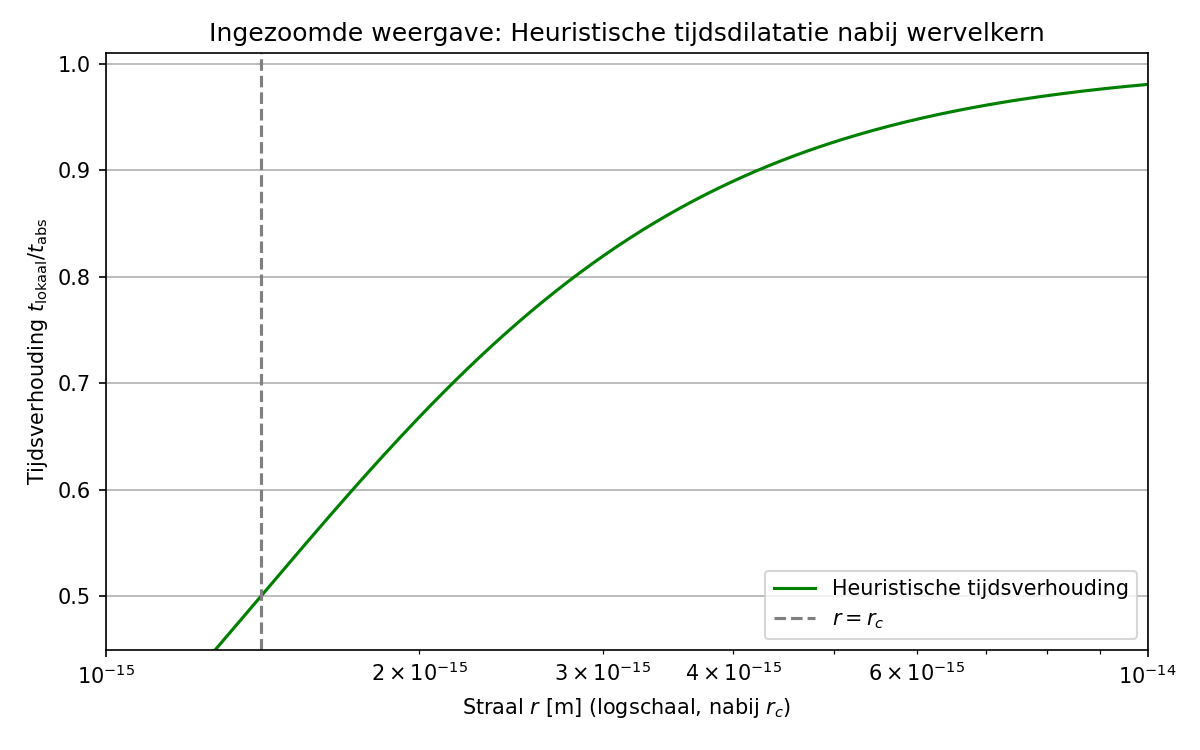
\includegraphics[width=0.7\textwidth]{images/06-HeuristicTimeDilation4_nl}
    \caption{
        Ingezoomd radiaal profiel van vortex-geïnduceerde tijddilatatie nabij de kern.
        Deze heuristische grafiek illustreert hoe de genormaliseerde lokale kloksnelheid
        $\frac{d\tau}{dt}$ snel toeneemt met de afstand $r$ tot de kern,
        en asymptotisch één nadert. Dit visualiseert direct het effect van
        de tangentiële vortexsnelheid $v_\varphi(r) \sim \kappa / r$ op de lokale tijdsverloop,
        zoals voorspeld door vergelijking~\eqref{eq:vortex_tijd_expliciet}.
    }
    \label{fig:HeuristicTimeDilation}
\end{figure}

\subsection{Afleiding vanuit wervel hydrodynamica}

De afleiding volgt uit het Bernoulli-principe voor een ideale vloeistofstroming, gegeven door:
\begin{equation}\label{eq:Bernoulli}
    P + \frac{1}{2}\rho_\text{\ae} v^2 = \text{constant}
\end{equation}

Met wervel-stroming geïntroduceerd via vorticiteit $\vec{\omega} = \nabla \times \vec{v}$, definieert de lokale drukverlaging ten opzichte van de verre omgeving een lokale tijdvertraging. De lokale wervelsnelheid is gegeven door:
\begin{equation}\label{eq:tangentiele_snelheid}
    v_{\phi}(r) = \frac{\Gamma}{2\pi r} = \frac{\kappa}{r}
\end{equation}

waarbij $\Gamma$ de circulatieconstante is, en $\kappa$ het circulatiekwantum. Substitutie van \eqref{eq:tangentiele_snelheid} in \eqref{eq:vortex_tijddilatatie} geeft expliciet:
\begin{equation}\label{eq:vortex_tijd_expliciet}
    \frac{d\tau}{dt} = \sqrt{1 - \frac{\kappa^2}{c^2 r^2}}
\end{equation}

Hiermee is de tijddilatatie expliciet uitgedrukt in fundamentele wervel-parameters.

\begin{figure}[H]
  \centering
  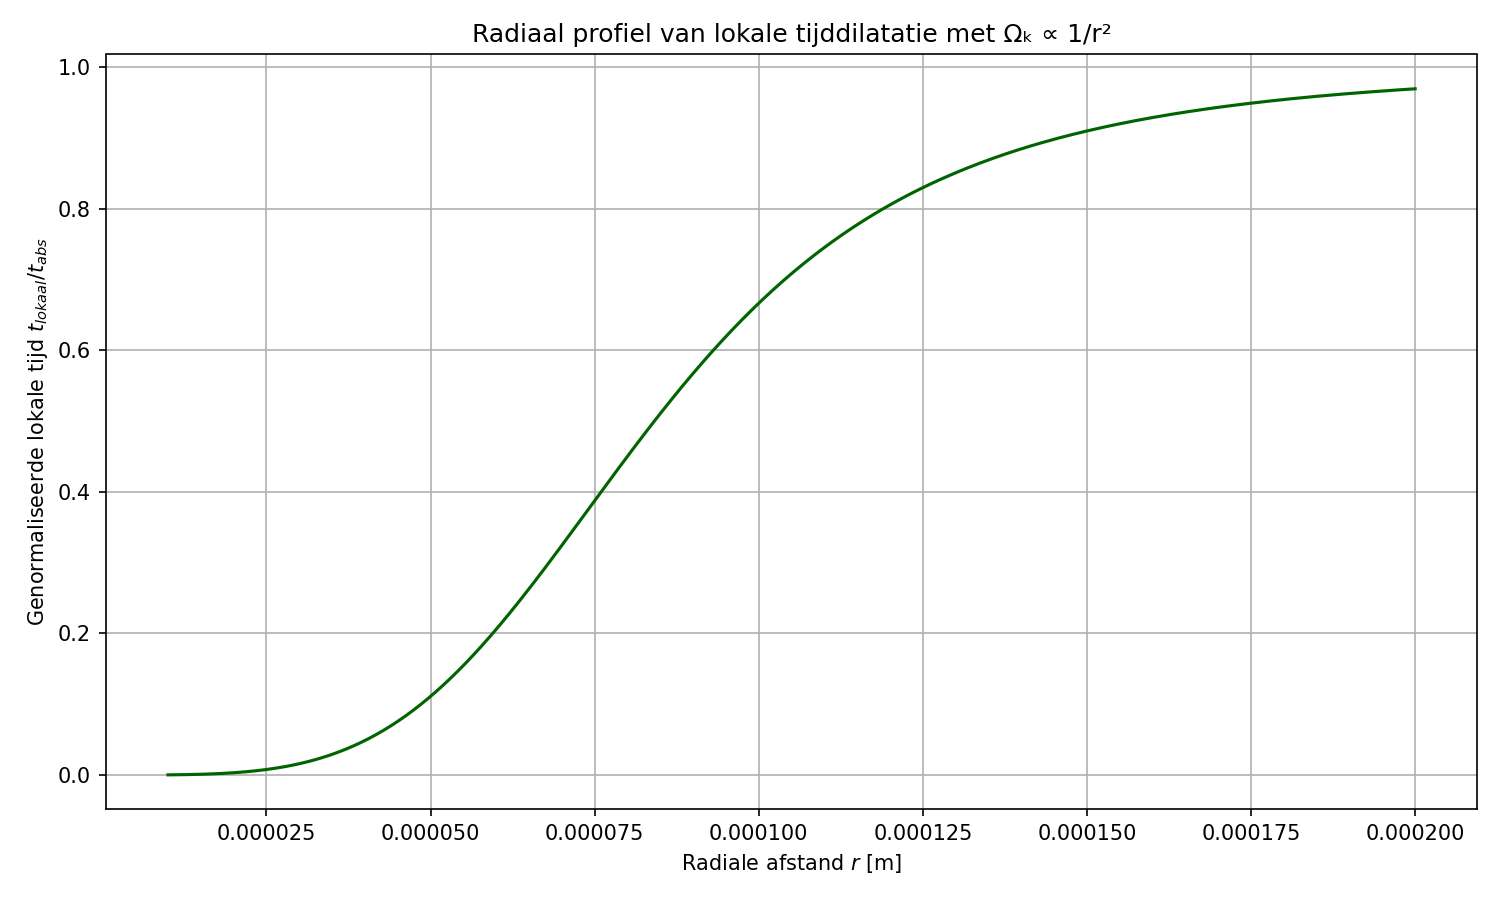
\includegraphics[width=0.7\textwidth]{images/02-RadialProfileOfLocalTimeDilation_Radial_LocalTime_Dilation_nl}
  \caption{Radiaal profiel van tijddilatatie als gevolg van wervelrotatie \( v_\varphi(r) = \kappa / r \). De lokale klokfrequentie neemt af met \(1/r^2\) en nadert asymptotisch 1 op grote afstand.}
  \label{fig:radiale_tijddilatatie}
\end{figure}


\subsection{Vergelijking met algemene relativiteit}

Ter vergelijking, in algemene relativiteit (GR) ontstaat gravitationele tijddilatatie uit ruimtetijdkromming, uitgedrukt door de Schwarzschildmetriek~\cite{schutz2009first}:
\begin{equation}\label{eq:GRtijd}
    \frac{d\tau}{dt} = \sqrt{1 - \frac{2GM}{rc^2}}
\end{equation}


De overeenkomsten en verschillen zijn direct zichtbaar: GR's gravitationele tijddilatatie is gerelateerd aan massa $M$ en gravitatieconstante $G$, terwijl VAM tijddilatatie puur hydrodynamisch is en direct verbonden met de lokale rotatiesnelheid van het æther medium via wervel-circulatie $\kappa$.

\begin{figure}[ht!]
    \centering
    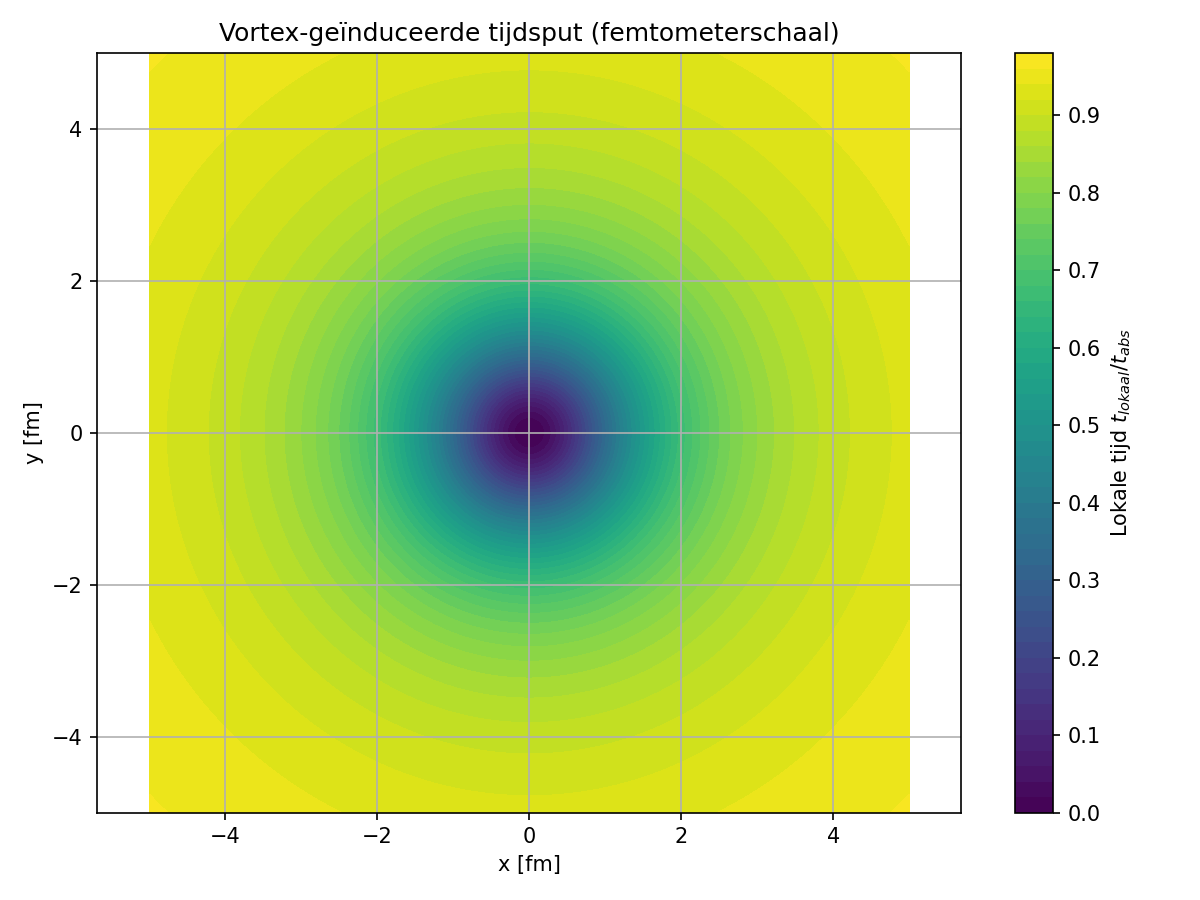
\includegraphics[width=0.7\linewidth]{images/02-RadialProfileOfLocalTimeDilation_Vortex-Induced_Time_Well_nl}
    \caption{Vergelijking tussen VAM- (vortex dynamiek) en GR-tijddilatatie, als functie van afstand tot wervelkern en Schwarzschildradius.}
    \label{fig:vergelijking_VAMGR}
\end{figure}

In Figuur~\ref{fig:vergelijking_VAMGR} zien we dat de VAM-tijddilatatie functioneel vergelijkbaar is met GR-prediction bij voldoende afstand. Bij afnemende afstand (nabij wervelkern of Schwarzschildradius) ontstaan verschillen door wervel-specifieke effecten en topologische knoopstructuren.

Samenvattend vervangt het VAM ruimtetijdkromming door werveldynamica, met behoud van meetbare tijddilatatie-effecten die overeenstemmen met gevestigde experimentele resultaten zoals Hafele–Keating~\cite{hafele1972around}, maar vanuit een fundamenteel andere fysische verklaring.


Ter illustratie vergelijken we in Figuur~\ref{fig:vergelijkingVAMGR} VAM en GR expliciet voor een neutronenster met $M = 2\,M_\odot$ en radius $R = 10\,\text{km}$. De verschillen worden duidelijk nabij de oppervlakte van het object, waar wervel-specifieke effecten optreden.

\begin{figure}[ht!]
    \centering
    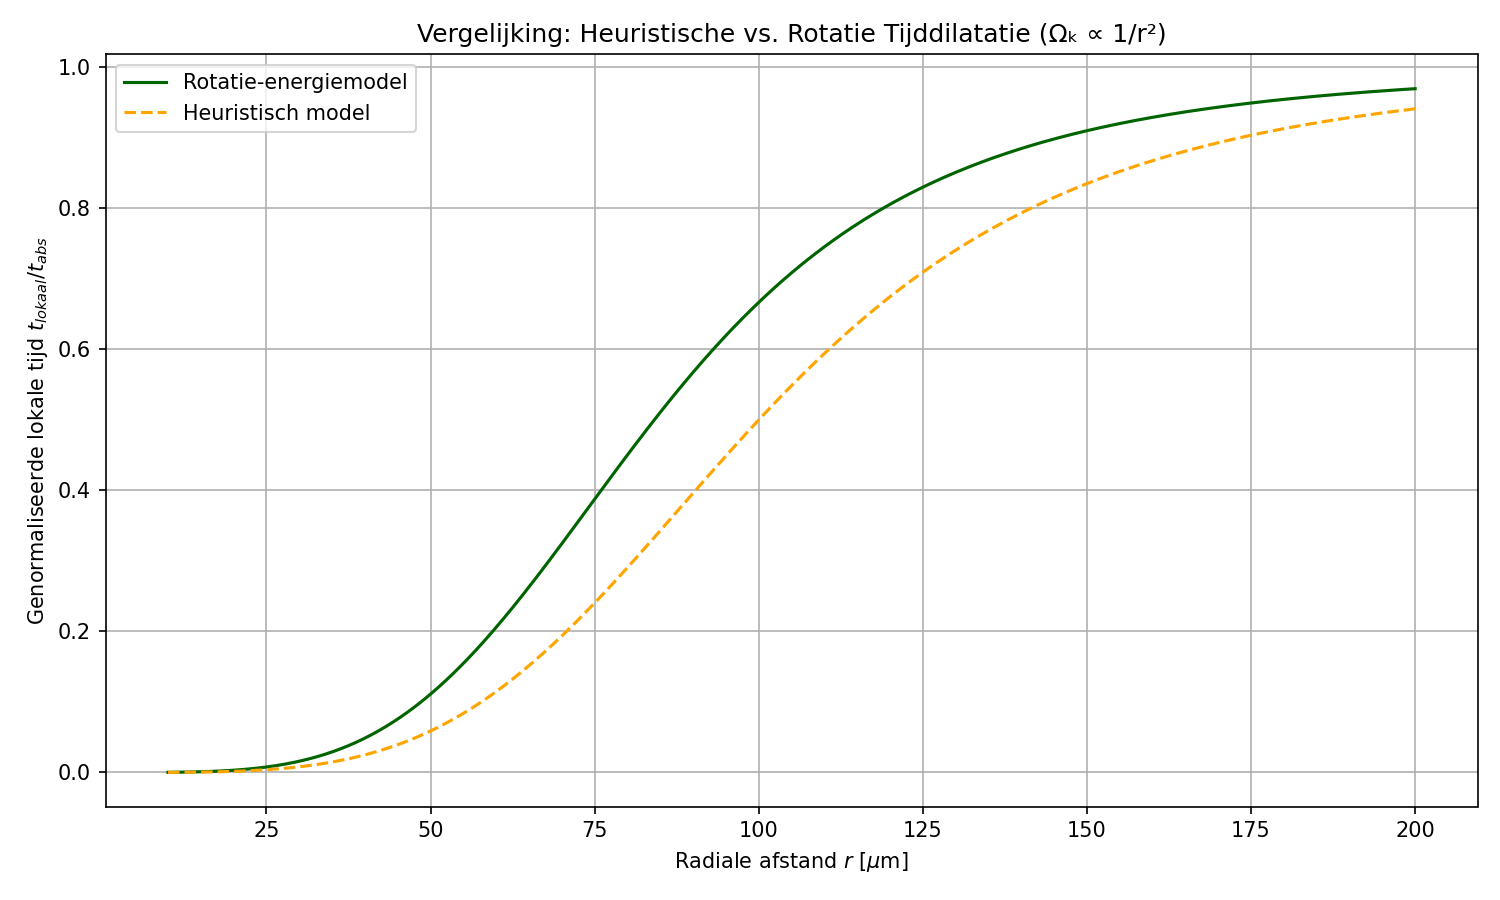
\includegraphics[width=0.7\linewidth]{images/04-RotationalVsHeuristicTimeDilation_nl}
    \caption{Verschil tussen VAM en GR-tijddilatatie voor een neutronenster ($2\,M_\odot$, $R=10$ km).}
    \label{fig:vergelijkingVAMGR}
\end{figure}


\subsection{Praktische implicaties en experimentele toetsbaarheid}

Een praktische implicatie van wervel-geïnduceerde tijddilatatie is dat klokken dicht bij intense wervelvelden meetbaar trager zouden lopen. Dit kan theoretisch getoetst worden met ultra-precieze atoomklokken in laboratorium wervelexperimenten, of indirect via astrofysische observaties van pulsars en neutronensterren. Het Hafele–Keating experiment biedt een directe analogie voor tijddilatatie door beweging en hoogteverschillen, die in VAM overeenkomt met lokale wervelvariaties~\cite{hafele1972around}.

\begin{figure}[ht!]
    \centering
    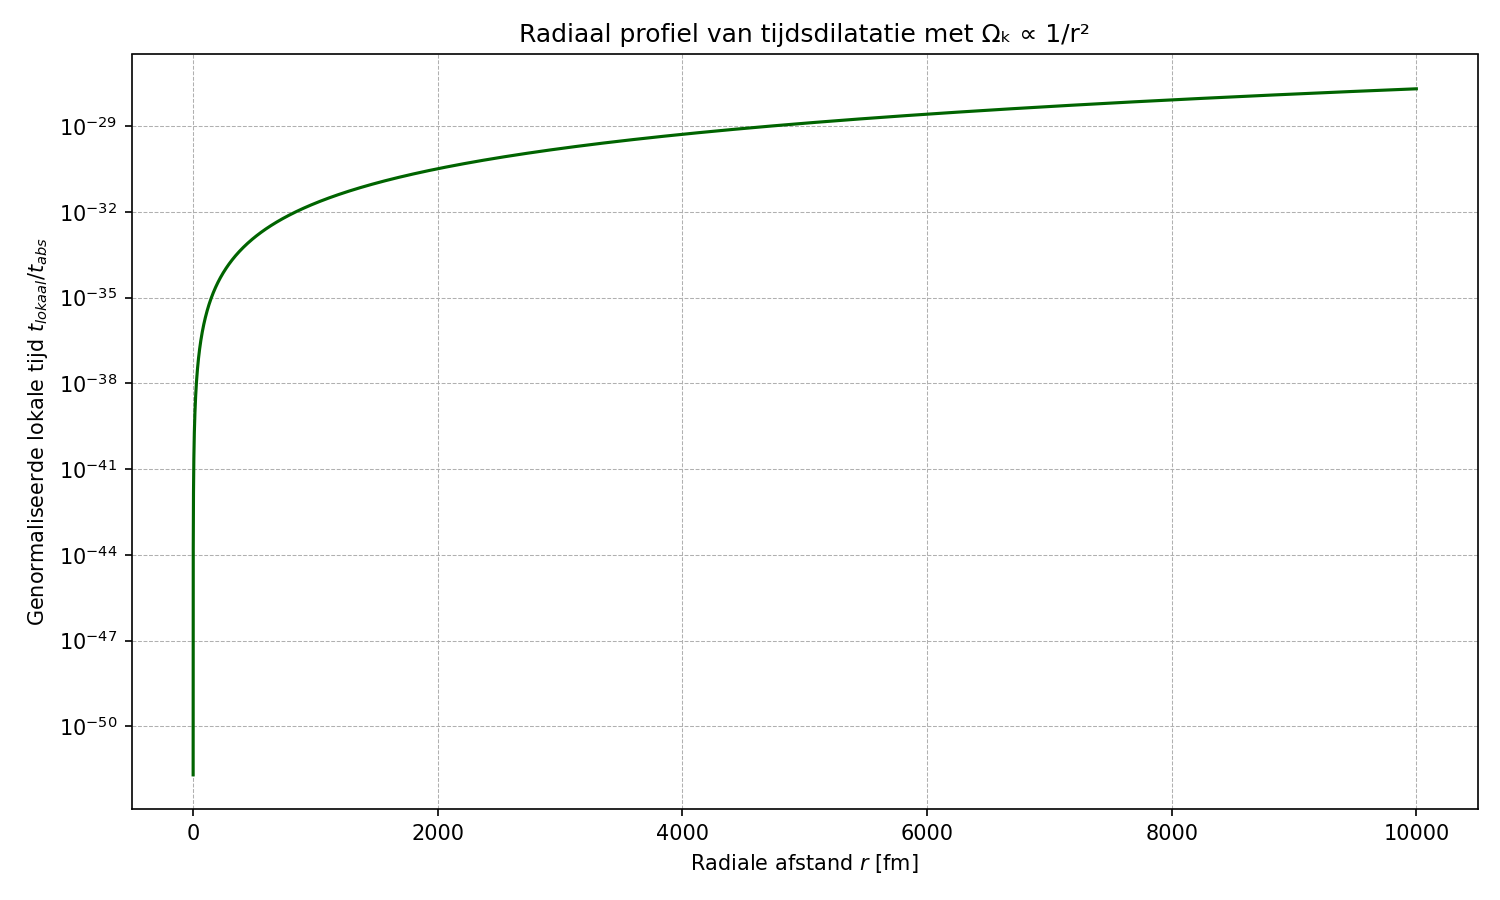
\includegraphics[width=0.7\linewidth]{images/05-LogarithmicDecayLocalTime_nl}
    \caption{Uitgebreid radiaal profiel van tijddilatatie met $\Omega_k \propto 1/r^2$, dat de diepe tijdsput-karakteristieken van wervelvelden op grote straal toont.}
    \label{fig:NewGraph}
\end{figure}